\documentclass[11pt]{article}\pagestyle{plain}
\usepackage{geometry}
\usepackage{graphicx}
\usepackage{caption}
%\usepackage{flexisym}
\usepackage{graphicx, subfig}
\usepackage{bbm}
\usepackage{CJK}
\usepackage{enumerate}
\usepackage{enumitem}
\usepackage{color}
%\usepackage{amsmath}
\usepackage{amssymb}
\usepackage{amsthm}
\usepackage{bm}
\usepackage{mathrsfs}
\usepackage{algorithmic,algorithm}
\usepackage{mathtools}
\newcommand{\red}[1]{\textcolor{red}{#1}}
\usepackage{amsmath}
\geometry{left=1in,right=1in,top=1in,bottom=1in}

\usepackage{url}

\usepackage{hyperref}

\linespread{1}
\setlength{\parskip}{1em}



% \usepackage{times}
% \oddsidemargin  0pt
% \evensidemargin 0pt
% \marginparwidth 0pt
% \topmargin    0pt
% \headheight   0pt
% \headsep      0pt
% \textwidth  470pt
% \textheight 630pt

% \usepackage{graphicx} 
% \usepackage{float}

% \usepackage{amsmath}
\DeclareMathOperator*{\argmax}{arg\,max}
\DeclareMathOperator*{\argmin}{arg\,min}

\usepackage{xcolor}
\newcommand\todo[1]{\textcolor{red}{#1}}

\def\R{\mathbb{R}}
\def\E{\mathbb{E}}
\def\P{\mathbb{P}}
\def\Cov{\mathrm{Cov}}
\def\Var{\mathrm{Var}}
\def\half{\frac{1}{2}}
\def\th{\mathrm{th}}
\def\tr{\mathrm{tr}}
\def\df{\mathrm{df}}
\def\dim{\mathrm{dim}}
\def\col{\mathrm{col}}
\def\row{\mathrm{row}}
\def\nul{\mathrm{null}}
\def\rank{\mathrm{rank}}
\def\nuli{\mathrm{nullity}}
\def\spa{\mathrm{span}}
\def\sign{\mathrm{sign}}
\def\supp{\mathrm{supp}}
\def\diag{\mathrm{diag}}
\def\aff{\mathrm{aff}}
\def\conv{\mathrm{conv}}
\def\hy{\hat{y}}
\def\ty{\tilde{y}}
\def\hbeta{\hat{\beta}}
\def\tbeta{\tilde{\beta}}
\def\htheta{\hat{\theta}}
\def\halpha{\hat{\alpha}}
\def\hf{\hat{f}}
\def\hmu{\hat{\mu}}
\def\hlambda{{\hat{\lambda}}}
\def\heta{{\hat{\eta}}}
\def\hR{{\widehat{R}}}
\def\cA{\mathcal{A}}
\def\cB{\mathcal{B}}
\def\cD{\mathcal{D}}
\def\cE{\mathcal{E}}
\def\cF{\mathcal{F}}
\def\cG{\mathcal{G}}
\def\cK{\mathcal{K}}
\def\cH{\mathcal{H}}
\def\cI{\mathcal{I}}
\def\cM{\mathcal{M}}
\def\cN{\mathcal{N}}
\def\cP{\mathcal{P}}
\def\cS{\mathcal{S}}
\def\cT{\mathcal{T}}
\def\cW{\mathcal{W}}
\def\cX{\mathcal{X}}
\def\cY{\mathcal{Y}}
\def\cZ{\mathcal{Z}}

% \usepackage{amssymb}

\newcommand{\yw}[1]{\textit{\textcolor{blue}{[yuxiang]: #1}}} % YW's notes

\begin{document}
\begin{center}\textbf{{\LARGE Homework 2 of CS 291K (Fall 2022)}\\[.3in]}

{\large University of California, Santa Barbara}\\[.3in]
%{\large Please attempt the problems.}\\[.1in]
{\large Due on Oct 27, 2022 (Thursday)}\\[.1in]
\end{center}
\rule[-10pt]{16.5cm}{0.05em} \\ 
\newline
\textbf{Notes:}
\vspace{-1em}
\begin{itemize}
\item You are welcome to discuss with your peers or the TAs if you run into challenges, but you need to declare any such discussion and everyone needs to write their own solutions independently.
\item You may refer to the matrix cookbook for matrix calculations: \url{https://www2.imm.dtu.dk/pubdb/edoc/imm3274.pdf}
\end{itemize}
\vspace{-2em}
\rule[-10pt]{16.5cm}{0.05em} \\


\paragraph{Problem 1. Feed-forward Neural Network}  (35') 


Let's consider a simple two layer neural network for binary classification. 

\begin{gather*}
	z_1 = W_1x^{(i)} + b_1\\
	a_1 = ReLU(z_1)\\
	z_2 = W_2 a_1 + b_2\\
	\hat{p}^{(i)} = \sigma(z_2)\\
	L^{(i)} = y^{(i)}*\log(\hat{p}^{(i)}) + (1- y^{(i)})*\log(1 - \hat{p}^{(i)})\\
	J = -\frac{1}{m} \displaystyle \sum_{i=1}^{m}L^{(i)}\\
\end{gather*}
It has input size $2\times 1$, one hidden layer size $3\times 1$, and output size $1$. $\sigma(\cdot)$ is the Sigmoid function.


The weights of the network are: 
$
W_1=
\begin{bmatrix}
	-0.2 & 0.1\\
	0.5 & 0.3\\
	0.35 & 0.4
\end{bmatrix}
$,
$
W_2=
\begin{bmatrix}
	1.5 & 0.6 & -0.4
\end{bmatrix}
$,

and biases
$
b_1=
\begin{bmatrix}
	1.2\\
	0\\
	-0.7
\end{bmatrix}
$,
$
b_2=
\begin{bmatrix}
	0.5
\end{bmatrix}
$, 

Assuming the network takes an input of 
$
x=
\begin{bmatrix}
	1.5\\
	-0.8
\end{bmatrix}
$, 

and the ground-truth label $y=0$.

\begin{enumerate}
	\item (5') What is the network prediction $\hat{p}$?
	\item (5') What is ${\partial J}$ / ${\partial \hat{p}}$?
	\item (5') What is ${\partial \hat{p}^{(i)}}$ / ${\partial z_2}$?
	\item (5') What is ${\partial z_2}$ / ${\partial a_1}$?
	\item (5') What is ${\partial a_1}$ / ${\partial z_1}$?
	\item (5') What is ${\partial z_1}$ / ${\partial W_1}$?
	\item (5') What is ${\partial J}$ / ${\partial W_1}$? Be careful with the shapes. 
\end{enumerate}


\paragraph{Problem 2. Convolutional Neural Network} (30')
\begin{enumerate}
	\item (5') Given an image of size $64\times 64$, what is the output dimension after applying a convolution with kernel size $5\times 5$, stride of 2, and no padding?
	
	\item (5') Given an input of dimension $C\times H\times W$, what is the output dimension of a convolutional layer with kernel size $K\times K$, padding $P$, stride of $S$, and $F$ channels (also called filters)?
	
	\item Suppose we have one batch 100 input images each of size $3\times 64\times 64$. Consider a convolutional layer with 2 output channels, kernel size $5\times 5$, no padding, and stride of 2. Answer the following questions and given brief explanations for your answers.
	
	\begin{enumerate}
		\item (5') What is the shape of the weight parameters for the convolutional layer?
		\item (5') What is the output size after we feed the whole batch of input images through the convolutional layer?
		\item (5') We decide to add a linear layer after the convolutional layer to make a prediction of whether the image contains a pedestrian, what would be the input dimension for the linear layer?
 	\end{enumerate}
 
 	\item (5') What is the purpose of a batch normalization layer in CNN?
\end{enumerate}


\paragraph{Problem 3. Transformer} (25' + 5')
\begin{enumerate}
	\item (5') What is the purpose of positional embedding in Transformer?
	\item (5') Why does Transformer need scaling factor for attention?
	\item (5') Consider the following Transformer for text generation with 3 encoding layers and 2 decoding layers. The embedding size is 64. The FFN hidden dimension is 256. It uses 8 heads. The max sequence length is 512. The shared vocabulary size is 4000. What is the total number of parameters? 
	\item (5') For the above model, suppose we use a minibatch size of 16. What is the running memory requirement for one step of SGD?
	\item (5') What is the training objective in BERT?
	\item (bonus 5') Can one use the BERT model to generate text? 
\end{enumerate}

\paragraph{(Bonus) Problem 4. Image Classification} (50+10')

The CIFAR-10~\footnote{\url{https://www.cs.toronto.edu/~kriz/cifar.html}} dataset is a widely used dataset for benchmarking image classification models. It consists of \textit{color} or RGB images taken from ten classes: airplane, automobile, bird, cat, deer, dog, frog, horse, ship, and truck. The classes are completely mutually exclusive. There is no overlap between automobiles and trucks. ``Automobile" includes sedans, SUVs, things of that sort. ``Truck" includes only big trucks. Neither includes pickup trucks. A few randomly drawn samples from the dataset are depicted in Figure~\ref{fig1}.

\begin{figure}[h]
	\centering
	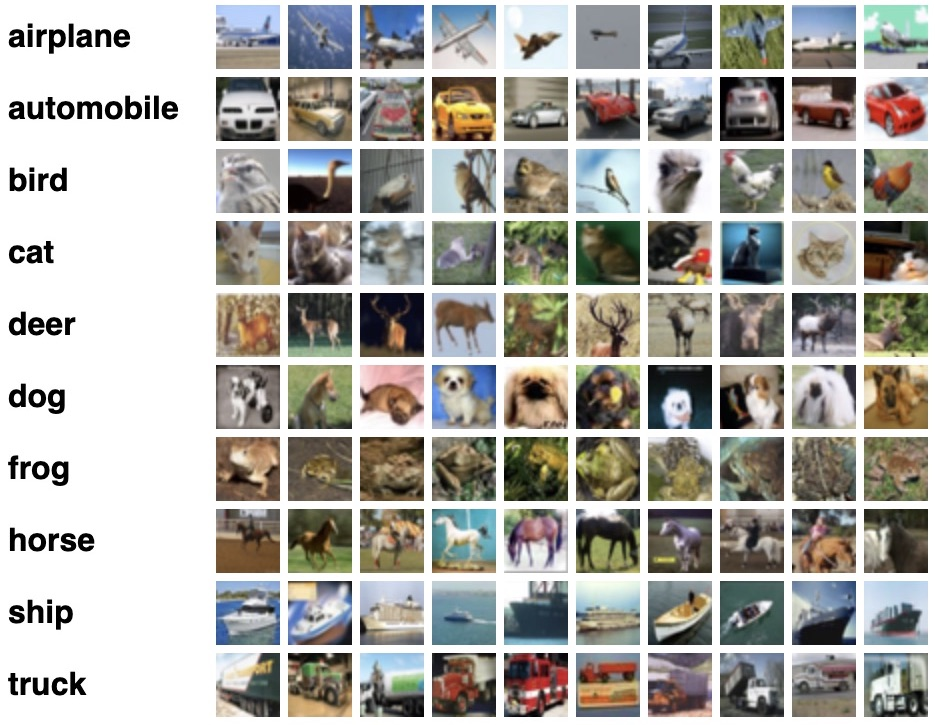
\includegraphics[height=3in]{CIFAR-10.jpg}
	\caption{Samples from the CIFAR-10 dataset.}
	\label{fig1}
\end{figure}

In this homework, you'll be training a deep learning model on this dataset, making predictions on unseen RGB images, and submitting your predictions on Kaggle. 
You may choose any neural network architecture. The network should NOT be pre-trained on external data. 


(Hint) To get the best performance out of a neural network (e.g. CNNs), there are two aspects you have to consider:
\begin{enumerate}
	\item \textbf{Model architecture} - Try different parameters for the conv layers, i.e, the number of channels, size and stride of the kernel, etc. Try different numbers of convolutional, pooling and fully connected layers. Add dropout and batch normalisation, anything else you can think of.
	\item \textbf{Optimization procedure} - Try different learning rates, L1/L2 regularization, different optimizers, different batch sizes and number of epochs, etc. 
\end{enumerate}

\textbf{Kaggle Competition}: \url{https://www.kaggle.com/competitions/ucsb-cs291k-hw2-2022-fall}
Join the competition. Start working on this homework by creating a new Kaggle notebook from the Code menu option and uploading the baseline. Enable GPU access using the accelerator option from the settings if needed. Alternatively, you can create a conda environment and develop the code on your local machine. Just like the previous homework, the baseline Ipynb notebook, python code, and conda environment files have been provided to you. Make sure to follow the correct procedure for running on Kaggle or your local machine. 

\paragraph{Code.} In addition to making submissions on the competition website, you need to submit your code either in \verb|.py| or \verb|.ipynb| format to Gradescope. Your code should run as is and should produce the exact same results as your submission on Kaggle.

\paragraph{Grading.} If the submitted code does not run out of the box, you would receive 0 pts regardless of the Kaggle competition score. Otherwise, your grade depends on the private accuracy score of your model predictions on Kaggle. The private leaderboard uses a different set of test examples to the public leaderboard and will only be revealed after the deadline. You should select one of your submissions as your final submission. The grading scheme is as following based on the accuracy on the private test set:

\begin{center}
	\begin{tabular}{rc}
		larger than 0 but lower than baseline (0.52): & 20 pts \\
		higher than baseline up to 0.64: & 40 pts \\
		higher than 0.64: & 50 pts \\
		top 10  on the private leaderboard and above 0.64: & +10 pts
	\end{tabular}
\end{center}

\end{document}
